\section{Circuito integratore}
\begin{figure}[h]
	\centering
	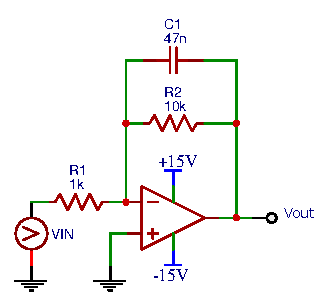
\includegraphics[scale=1]{integratore.pdf}
	\caption{circuito integratore con OpAmp.}
	\label{f:integratore}
\end{figure}
Si è montato il circuito in \ref{f:integratore} con $R_1= \SI{0.981(9)}{\kohm}$, $R_2= \SI{9.87(9)}{\kohm}$,$C_1= 48\pm2$nF. L'ampiezza picco-picco di $V_{in}=\SI{2.08(2)}{\V}$. Al variare della frequenza si è misurato $V_{out}$ con l'oscilloscopio. La frequenza è stata misurata con il frequenzimetro dell'oscilloscopio e lo sfasamento tra $V_{in}$ e $V_{out}$ si è ricavato dalla misura dell'intervallo di tempo $\Delta$T tra le due intersezioni delle onde in ingresso e uscita con l'asse delle ascisse \footnote{Tale asse orizzontale corrispomde per ogni onda ad una tensione costante pari al proprio valor medio}.Da questa misura si ricava lo sfasemento:$ \Delta\phi = 2\Delta$Tf.\\
Per quanto riguarda il guadagno in frequenza sono stati eseguiti due fit(in \ref{f:guad_integ}), uno nella parte piatta dei dati cioè a basse frequenze ed un altro ad alte frequenze per studiare i due limiti del circuito integratore, rispettivamente $f<<f_t$ e $f>>f_t$.
Per $f_t$ si intende la frequenza di taglio del circuito integratore pari a $f_t=\frac{1}{2\pi R_2C_1}= \SI{335(16)}{\Hz}$. \\
\\
Il fit a basse frequenze ($f< \SI{50}{\Hz}$) è stato eseguito con una costante e i risultati sono :\\
$A_v= \SI{20.05(2)}{}$\\
$\chi^2=4.79$ ($4$ dof, $p = 0.31$)\\
\\
Il fit ad alte frequenze ($f> \SI{2}{\kHz}$) è stato eseguito con una funzione lineare $A_v(dB)= a\log_{10} f +b$  e i risultati sono:\\
$a= \SI{-19.8(2)}{\frac{\dB}{\deca}}$\\
$b= \SI{69.9(4)}{\dB}$\\
$\chi^2=3.89$ ($5$ dof, $p = 0.56$)\\
\\
Il valore atteso del guadagno a basse frequenze è $A_v=20\log_{10} \frac{R_2}{R_1}= \ SI{20.1(2)}{dB}$ compatibile con il valore ottenuto dal fit.
Ad alte frequenze la pendenza della retta è compatibile con $\SI{-20}{\frac{\dB}{\deca}}$.\\
E' stato eseguito anche un fit allo sfasamento() con un modello non lineare $\Delta \phi= \arctan{\frac{-f}{f_t}}$ e si è ottenuto:\\
$f_t= \SI{321(2)}{\Hz}$\\
$\chi^2=62.21$ ($16$ dof, $p = 0$)\\
Il valore della frequenza di taglio risulta compatibile con quello atteso prima calcolato.\\
\\
Si è poi verificata la risposta del circuito ad un'onda quadra di frequenza $f= \SI{10.6(1)}{\kHz}$. Con un'ampiezza di $V_{in}=\SI{3.63(2)}{\V}$ si è ottenuta un'ampiezza di $V_{out}=\SI{1.90(2)}{\V}$ quindi $A_v=\SI{-5.6(2)}{\dB}$.
??????VALORE ATTESO QUAL E'????????

Dai grafici in \ref{f:integ1}, in \ref{f:integ3} e in \ref{f:integ5} si nota che all'aumentare della frequenza l'onda quadra viene sempre meglio integrata, soprattutto quando $f> f_t$. Tuttavia a frequenze molto elevate si nota che il tempo in cui l'onda quadra è alta o bassa è molto minore di quello necessario al condensatore per caricarsi, quindi la tensione ai capi di quest'ultimo rimane costante. \\
Il ruolo di $R_2$ è quello di stabilizzare il circuito integratore in modo che l'OpAmp non vada subito in saturazione se in ingresso c'è una componente continua.Inserendo tale resistenza il polo della funzione di trasferimento presente nello zero viene spostato in $-\frac{1}{R_2C_1}$.Così facendo si rimuove la divergenza del guadagno per frequenze nulle.

\begin{figure}[h]
	\centering
	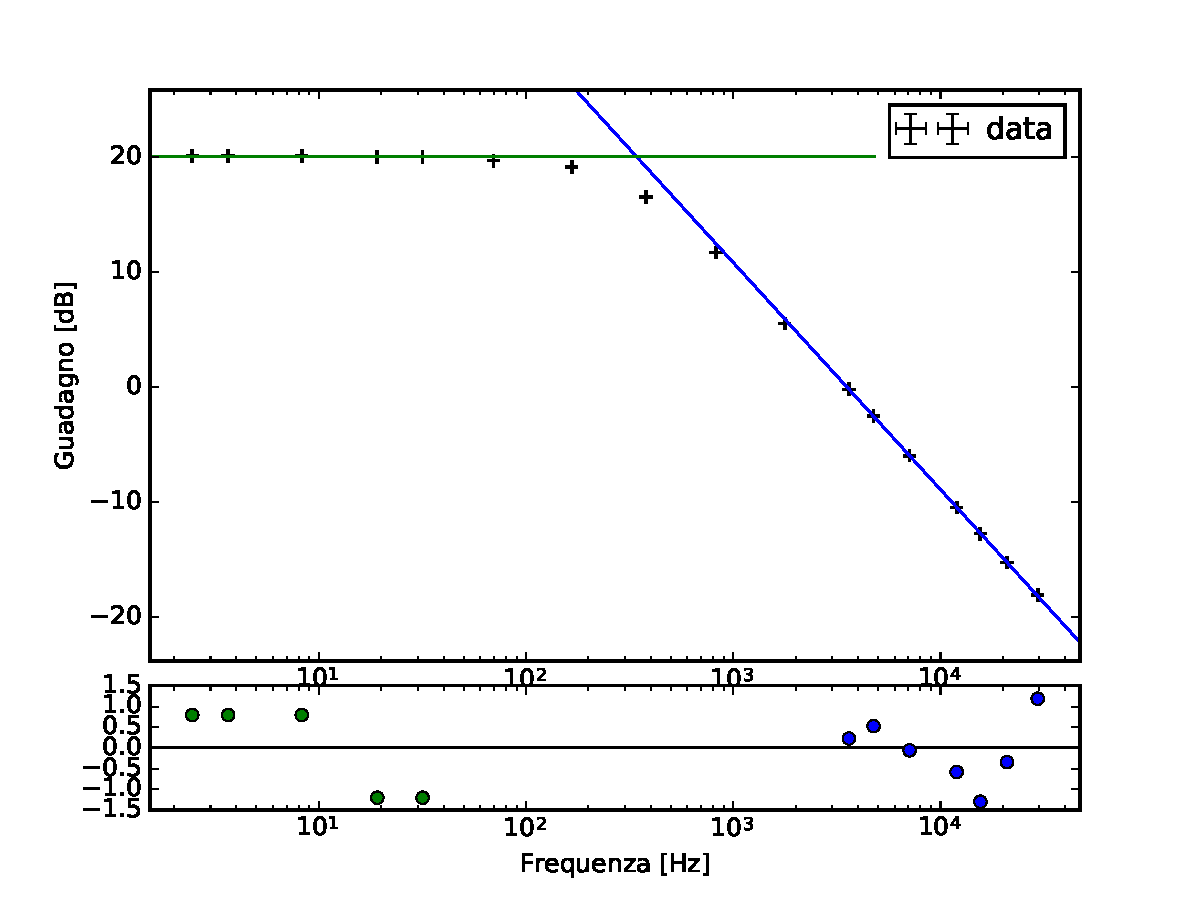
\includegraphics[scale=0.7]{fit_guad_integratore.pdf}
	\caption{plot di bode del guadagno del circuito integratore.}
	\label{f:guad_integ}
\end{figure}

\begin{figure}[h]
	\centering
	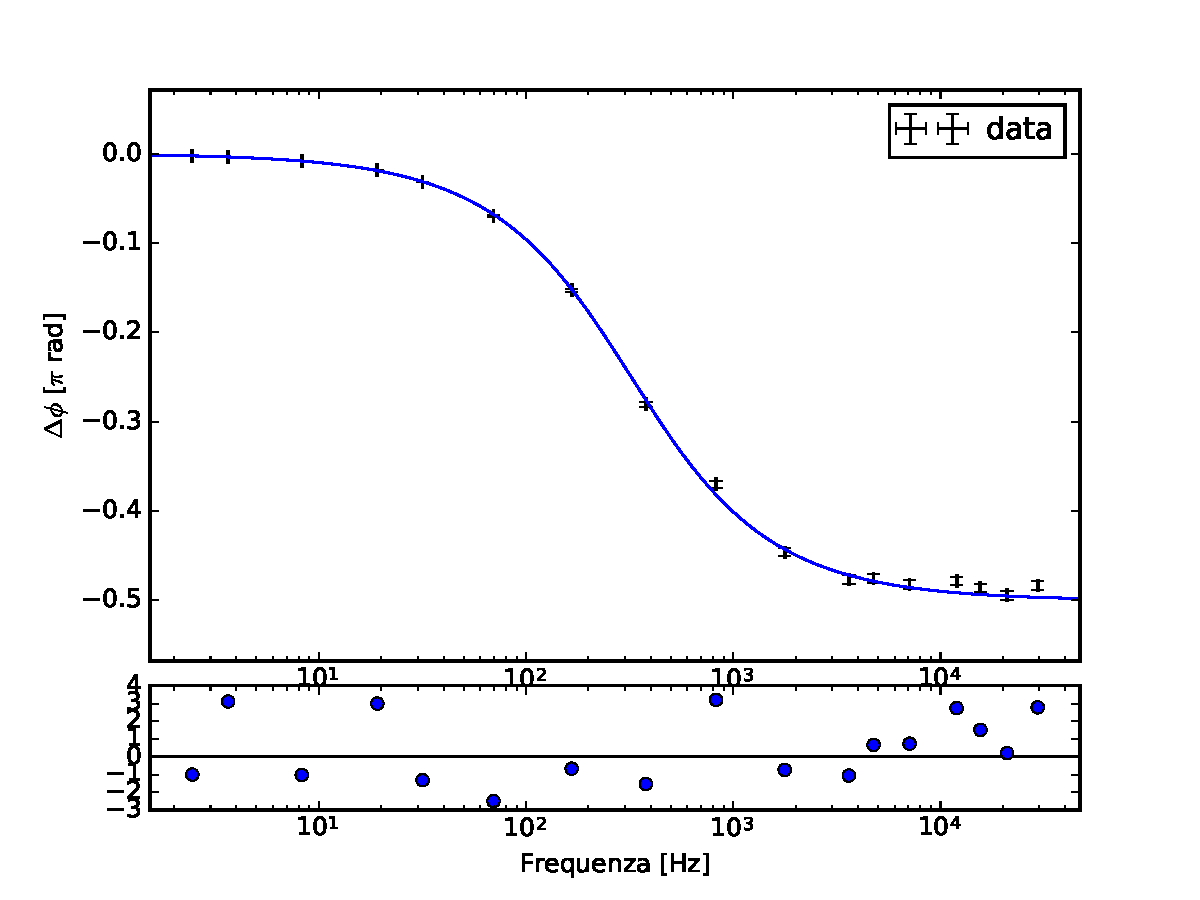
\includegraphics[scale=0.7]{fit_fase_integratore.pdf}
	\caption{fase in unità $\pi$ del circuito integratore in funzione della frequenza.}
	\label{f:fase_integ}
\end{figure}

\begin{figure}[h]
	\centering
	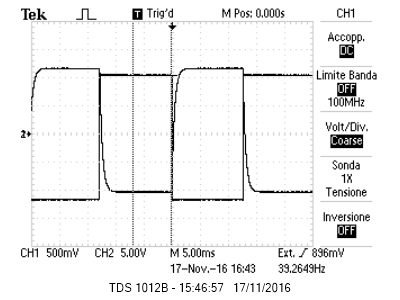
\includegraphics[scale=1]{data_integratore1.png}
	\caption{Risposta integratore ad un onda quadra di frequenza $\SI{39}{\Hz}$.}
	\label{f:integ1}
\end{figure}

\begin{figure}[h]
	\centering
	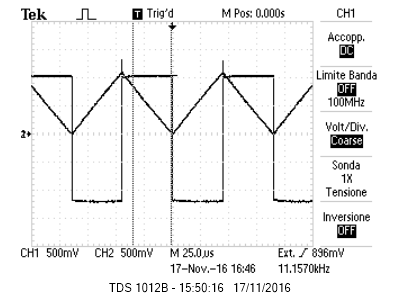
\includegraphics[scale=1]{data_integratore4.png}
	\caption{Risposta integratore ad un onda quadra di frequenza $\SI{11}{\kHz}$.}
	\label{f:integ3}
\end{figure}	

\begin{figure}[h]
	\centering
	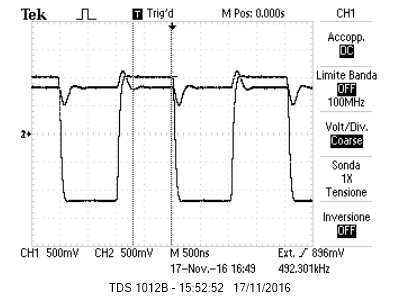
\includegraphics[scale=1]{data_integratore5.png}
	\caption{Risposta integratore ad un onda quadra di frequenza $\SI{492}{\kHz}$.}
	\label{f:integ5}
\end{figure}